\subsubsection{Preámbulo}

Los asistentes virtuales cada vez están más presentes en nuestras vidas gracias a todos los avances de la tecnología, y puede verse en que ya aparecen en todos los teléfonos móviles para ayudar en el día a día de los usuarios, ya sea para responder preguntas, poner una canción, o buscar información de manera rápida para el usuario.

La utilización de estos asistentes virtuales hace que cada vez más personas se planteen la posibilidad de llevar más lejos la utilización de ellos, como puede ser a través de otros dispositivos inteligentes a los que se les está buscando hueco cada vez en más hogares.

Estos dispositivos nos hacen la vida más sencilla, ayudando a actualizar y controlar toda la domótica de nuestras casas, de manera que se puedan realizar acciones en nuestra vivienda que hace unos años solo se podían imaginar en películas de ciencia ficción.

La utilización de asistentes virtuales para facilitar acciones que se repiten de manera continuada a lo largo de los días está cada vez más de moda: según un estudio de la reputada Nielsen~\cite{nielsen}, durante el Q2 de 2018 ha llegado a crecer el número de dispositivos desplegados en los hogares de Estados Unidos hasta alcanzar el 24\% de la población.

A la pregunta de para qué puede querer el 24\% de las familias un dispositivo asistente en sus casas, se puede observar tras una encuesta de dicho estudio, que en la mayoría de hogares se daba un uso bastante simple, solicitando al dispositivo únicamente la reproducción de contenido multimedia, pero esto ocurre únicamente en las primeras semanas de uso. También se puede observar en el estudio que, posteriormente, se tiende a dar más uso al dispositivo llegándole a requerir información habitual que se requiere de manera repetitiva cada semana, como puede ser la consulta del tiempo, la del tráfico antes de ir a trabajar o a la consulta de algún evento cercano importante.

La simplicidad de uso y todas las posibilidades que abarca ha hecho que una vez ha sido usado este tipo de dispositivo inteligente en cualquier hogar, se le siga utilizando cada vez para más tareas, dada su usabilidad y abanico de utilidades.

En ese estudio arriba citado, también se puede observar el comportamiento de los usuarios: una vez el dispositivo está en entre las cuatro paredes de la casa, se tiende a acompañar a este dispositivo inteligente de otros dispositivos domóticos, convirtiendo poco a poco el hogar en un sistema interconectado: cuatro de cada diez hogares disponen de más de un dispositivo inteligente en el hogar, y el 45\% de los hogares se plantean acompañar al que ya tienen, comprando otro.

Esta gran aceptación a la domótica viene dada gracias a la cantidad de variantes de las cuales podemos dotar al hogar, pudiendo ser todas controladas a través del dispositivo asistente, así como puede ser la programación de los tiempos de uso de aparatos como las bombillas, el termostato, los sistemas de seguridad, e incluso tanto el frigorífico, el sistema de riego, u otras acciones relativas a la seguridad de la vivienda como puede ser bloquear las puertas y ventanas, al igual que mantener el registro de cuáles y cuándo han sido abiertas, entre otras muchas opciones.

Al irrumpir estos dispositivos en las acciones cotidianas de un día corriente, se le permite al usuario adaptarse y ver que estos aparatos le acaban facilitando el día.

Viendo el creciente uso de estos dispositivos y las grandes marcas que hacen acto de presencia facilitando su implementación, entre las cuales se encuentran Google o Amazon, se puede pensar que este mercado ya está dominado y pertenece a estos dos grandes imperios, pero en este caso no se va a tener en cuenta todo lo que ya ofrecen, sino que se va a tener en cuenta todo lo que no están ofreciendo, o qué es lo que sus dispositivos no están preparados para ofrecer:

Como bien se ha visto, el punto de mira en todo el tema de la domótica y asistentes tiene un público objetivo que es el que pertenece a un rango de edad al que le gusta la tecnología y le parecería interesante automatizar las tareas del hogar, pero el verdadero público que podría exprimir todo su potencial es el público que menos acostumbrado nos tiene a estar a la vanguardia de la tecnología, el público perteneciente a la tercera edad.

Si se realiza el acto de volver a pensar sobre lo que es un asistente personal, en cuanto a una persona que trabaja como asistente, se entiende que es una persona que ayuda en las acciones del día a día más simples y repetitivas para las que otra persona no es capaz de hacer por si misma por algún tipo de incapacidad, ya sea incapacidad temporal, o algún tipo de incapacidad física.

Una vez planteado a qué se dedica un asistente personal, es fácil darse cuenta que al hablar de este trabajador se plasme la imagen de una persona que ayuda a personas mayores, o a personas con algún tipo de discapacidad.

El rango de personas de tercera edad es un público que puede necesitar que le levanten las persianas de manera automática porque quizá, le cuesta levantarse de la cama. Es un público que puede necesitar utilizar un asistente que le recuerde realizar ciertas tareas en su día a día como puede ser ir al médico, tomarse la pastilla, hacer la compra, o recordarle qué productos tiene que comprar, al igual que el cumpleaños de un ser querido. Todo esto acompañado de la seguridad que le puede proporcionar tareas como asegurarse que todas las puertas de su casa están bien cerradas, o saber que aún estando estas personas solas en casa, podrían solicitar auxilio en un momento de urgencia a través del asistente.

La tecnología vinculada a Internet nos hace la vida más sencilla a través del smartphone o de los ordenadores, pero las labores que nos proporciona como extra un dispositivo asistente inteligente a un usuario medio el cual ya está acostumbrado a usar un smartphone son muy pocas, ya que podría realizarlas a través de su propio teléfono, en cambio, a una persona de tercera edad a la cual le cuesta hacer un uso normal de dispositivos tecnológicos, un dispositivo asistente inteligente podría hacerle la vida mucho más sencilla, ya que lo único que necesitaría sería establecer una conversación oral con el dispositivo, evitando el intermediario que supone un ordenador o un smartphone.

El rango de personas de tercera edad, es por tanto el público que más puede necesitar un dispositivo asistente, así como el público que más puede llegar a exprimirlo.

La creación de un asistente que pueda resolver sus dudas, con el que pueda hablar, al que pueda preguntar a qué hora es la partida de cartas en el bar, o al que puedan pedir auxilio en caso de una caída, puede ser de gran utilidad para mejorar su día a día, al igual que servir de alivio para el resto de familiares que no pueden estar cerca de sus seres queridos, sabiendo que van a poder ser informados rápidamente de un posible accidente.

He aquí, por tanto, el agujero de mercado que ha sido encontrado en las grandes empresas antes nombradas, y el cual puede permitir un modelo de negocio el cual tenga como premisa buscar la satisfacción de las personas mayores, que igualmente puede servir para dar libertad a otros grupos sociales, como pueden ser las personas con algún tipo de discapacidad.

El auge de los dispositivos asistentes se puede ver como una evolución tecnológica que permita facilitar las rutinas, pero también con ello se pone en vilo la gestión de la privacidad e intimidad que hay dentro de nuestras casas. Esto es debido a que este tipo de dispositivos inteligentes pueden recolectar información a través de escuchar las conversaciones de un usuario y su día a día, siendo información que no se sabe de manera exacta a dónde va a parar, o qué se va a hacer con ella.

Esta información captada puede ser de un carácter sensible, ya que puede contener desde simples gustos, incluyendo las necesidades del usuario, como sus tendencias políticas, siendo datos que pueden estar siendo utilizados por terceros, o incluso pudiendo estar siendo vendidos.

La falta de soluciones en el mercado que cumplan todos estos puntos supone una motivación para la creación de un asistente que no esté conectado constantemente a Internet, ya que las personas de edad avanzada seguramente no tengan contratado el servicio, y que tampoco almacene datos de carácter sensible de los usuarios, sino que simplemente interaccione con cada persona y la ayude en su día a día, tanto ofreciendo actividades de la misma localidad, como respondiendo cualquier pregunta que pase por la cabeza de quien lo posea, al igual que buscando ayuda en caso de que una persona requiera auxilio.

Antes de adentrar en la elección de un asistente inteligente, se expondrá qué es, y cuál es su funcionamiento, para entender mejor los motivos por los cuales se acaba eligiendo uno en vez de otro.

\subsubsection{Qué es un Asistente Inteligente}

Un asistente inteligente es una máquina programada de tal manera que su comportamiento se asemeje al de una persona a la que se solicita asistencia, como su propio nombre indica, pudiendo mantener una conversación que siga los protocolos de comunicación humana.

\begin{figure}[h!]
    \centering
    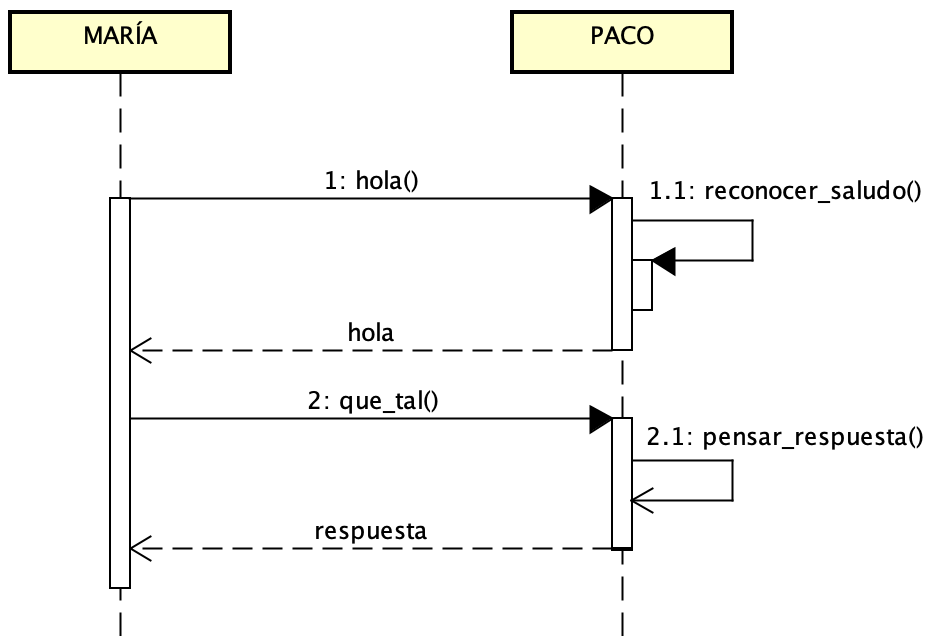
\includegraphics[width=10cm]{./img/sequence/human.png}
    \caption{Secuencia de Comunicación humana}
    \label{fig:humanseq}
\end{figure}

Como se puede ver en la figura \ref{fig:humanseq}, un protocolo de comunicación entre dos personas se basaría en un saludo para entablar conversación, para posteriormente realizar una pregunta.

En el caso de los asistentes, el proceso de conversación se basa en lo mismo: un usuario saluda al asistente mediante el uso de una palabra o conjunto de palabras, al que se llamará \textbf{hotword}, que cuando sea reconocido por el asistente inteligente, devolverá el saludo.
Es entonces cuando el usuario debe realizar la pregunta o solicitar la información que requiera.
Una vez hecha la pregunta, el dispositivo se pondrá a pensar la posible respuesta, entrando en el proceso al que se llamará \textbf{reconocimiento de los hechos}. Una vez identificados los hechos, devolverá la respuesta que más se acerque a lo deseado, gracias a un entrenamiento previo.

\newpage
\subsubsection{Cómo Piensa el Asistente}

El proceso de pensamiento analizado de los principales asistentes del mercado, que se expondrá en el presente capítulo, tiene una estructura similar independientemente del tipo de asistente que se trate, asemejándose a la figura \ref{fig:humasseq}.

\begin{figure}[h!]
    \centering
    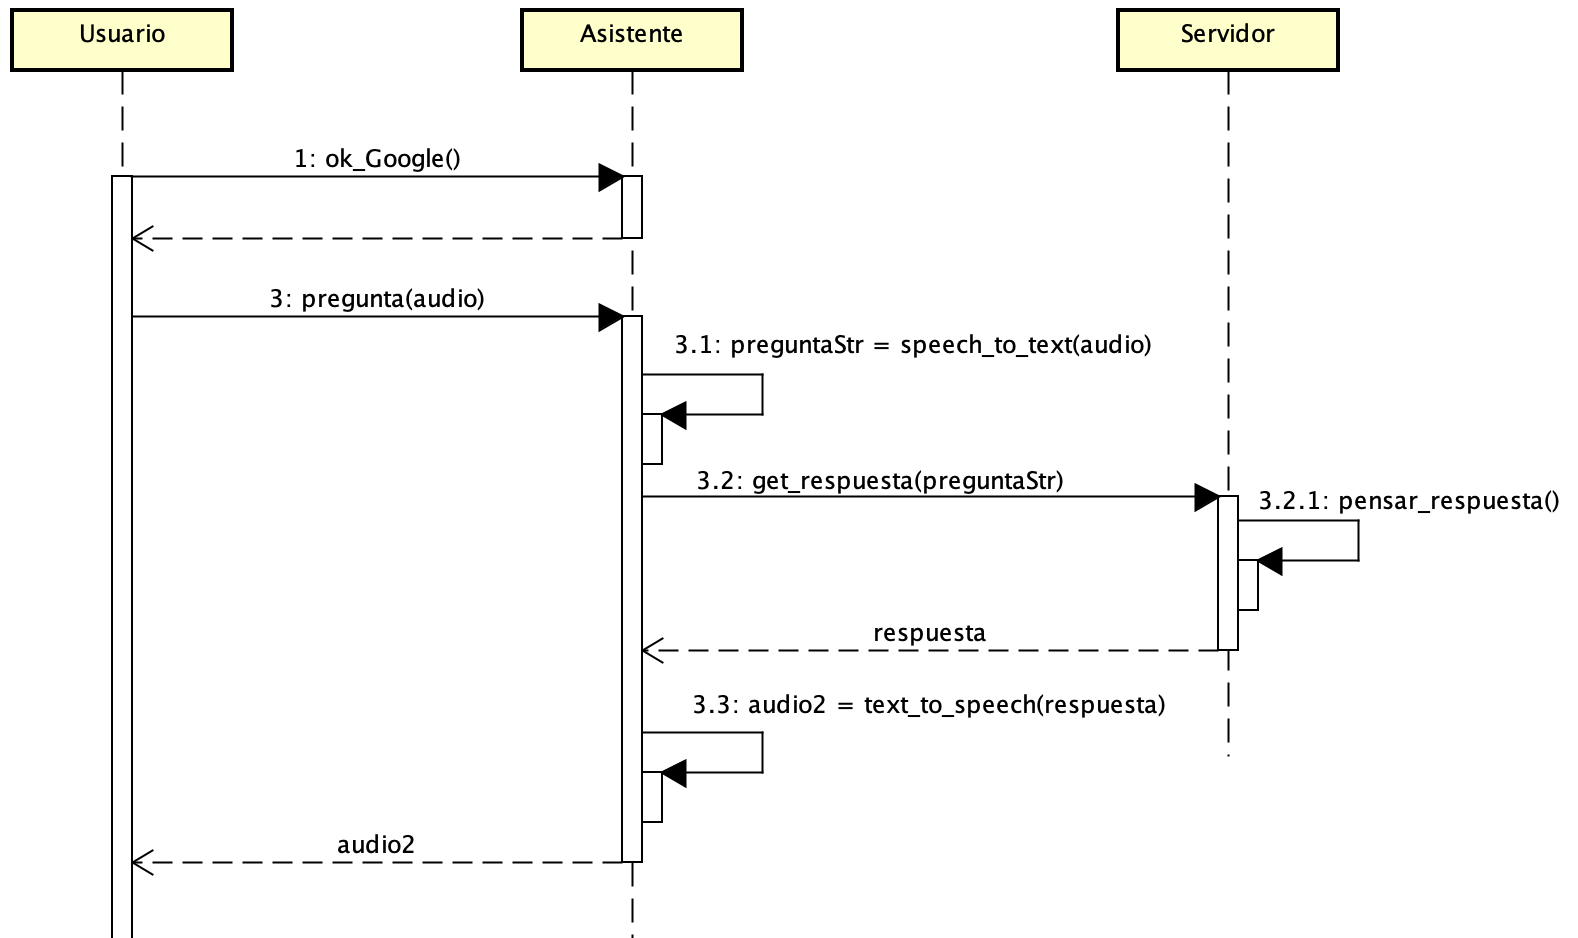
\includegraphics[width=13cm]{./img/sequence/humasseq.png}
    \caption{Secuencia de Comunicación humano-asistente}
    \label{fig:humasseq}
\end{figure}

Lo que diferencia a un asistente de otro, es la manera en la cual piensa la respuesta, dando mayor validez a un asistente que dé una respuesta más aproximada a lo solicitado.
Para lograr dar la respuesta más acertada, la mayoría de los asistentes existentes realizan el procesamiento de la respuesta en la nube debido a la gran cantidad de información que tienen previamente almacenada de otras consulta de otros usuarios para contrastar los hechos capturados, al igual que también pueden realizar en la nube el proceso de speech-to-text enviando los audios a sus servidores y transformándolo ahí a cadenas de texto, o el de text-to-speech, que sería el proceso inverso.
